\documentclass[msthesis.tex]{subfiles}

\begin{document}
\chapter{Results}
In this section, the quantitative and visualization results from the methods presented in \autoref{chap:methods} will be presented. The first two sections will present results from preprocessing of the \gls{DWI} images mentioned in \autoref{sec:Diffusionimgprepro} and extraction of connectivity matrices. The subsequent sections will statistically describe the nature of the data as well as classification results based on the comprehensive classification parameters illustrated in \autoref{tab:classify_combo}.

\section{Preprocessing Visualization}
\begin{figure}
    \centering
    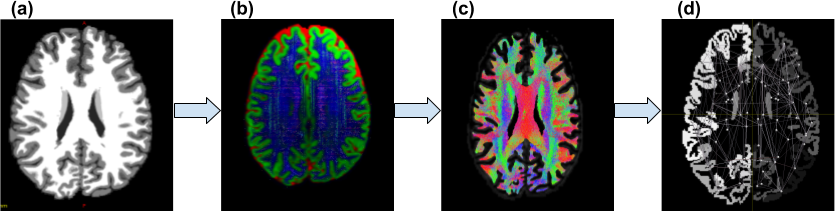
\includegraphics[width=\textwidth]{images/Preprocessing_pipeline.png}
    %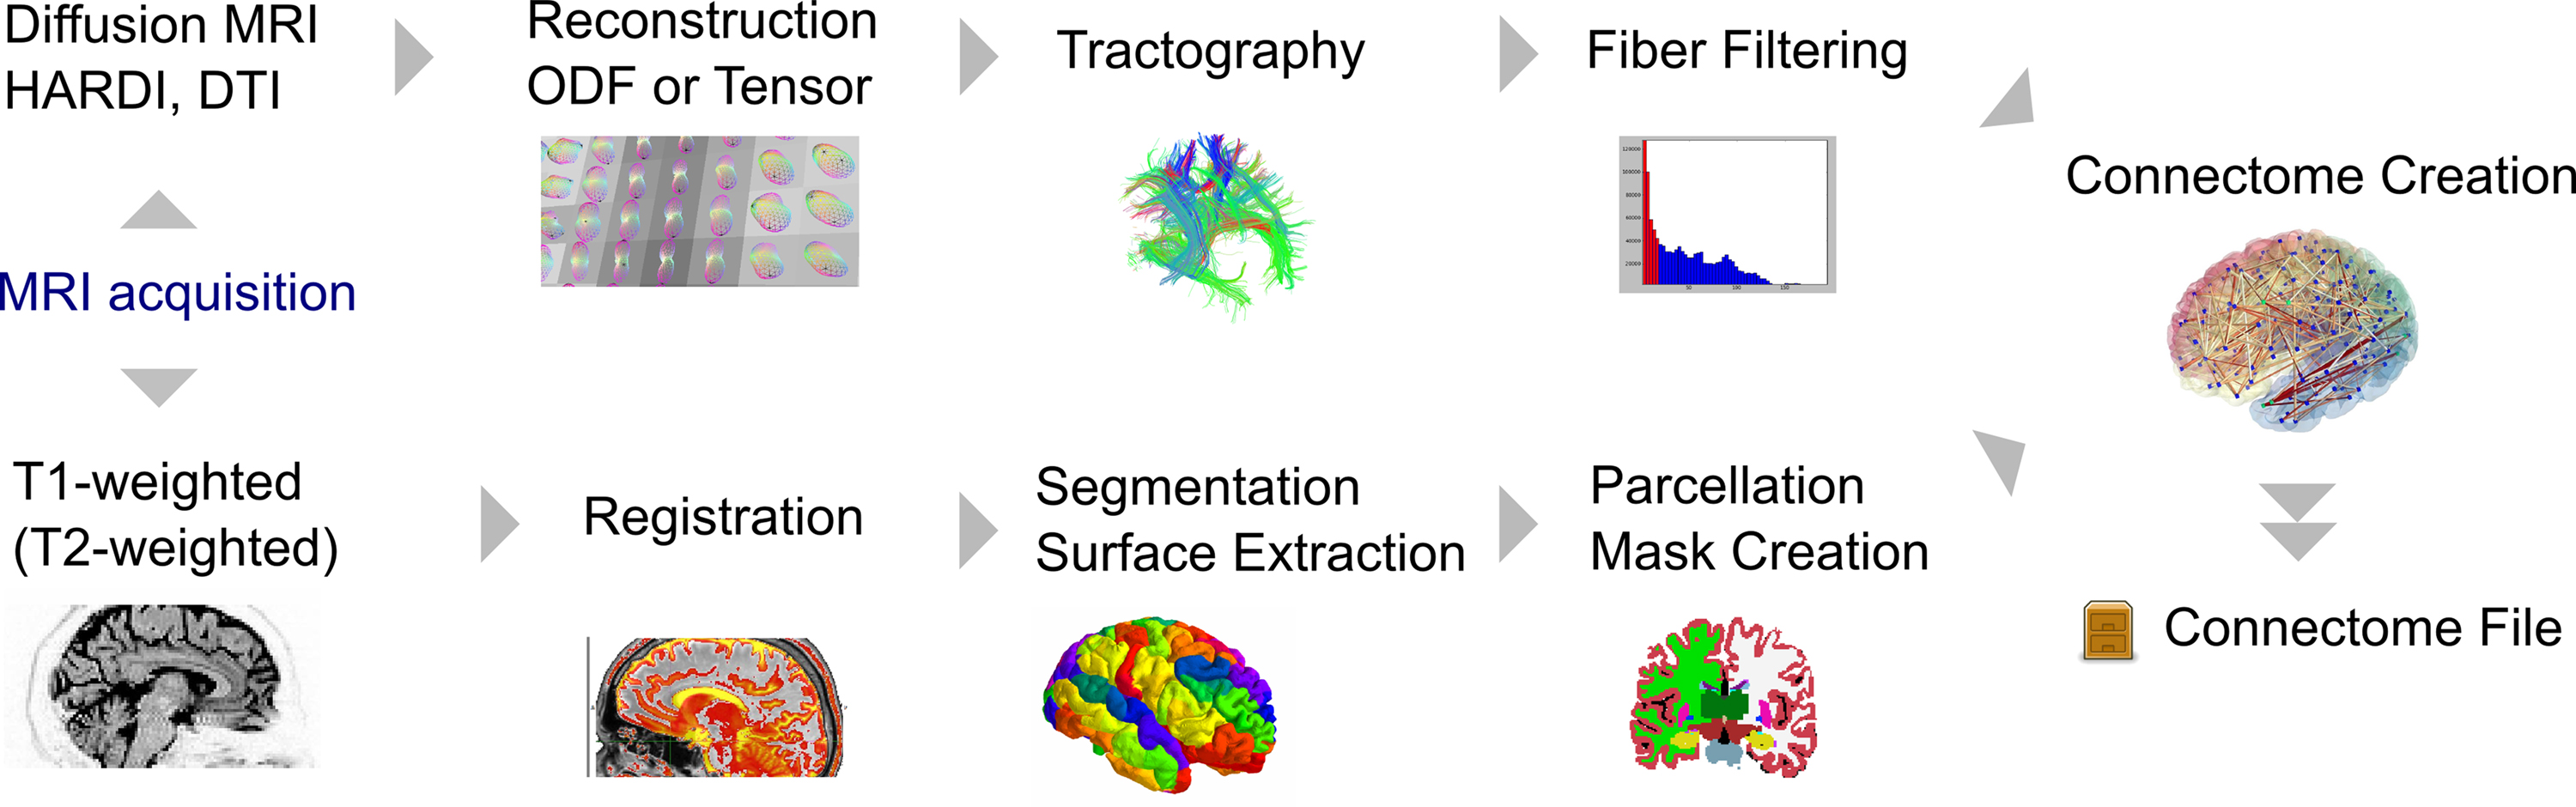
\includegraphics[width=\textwidth]{images/connectome_creation_workflow.png}
    %\cite{gerhard2011connectome}
    \caption{Visualization of pipeline used to create a connectome for each subject on an axial slice (a) Five tissue segmented image visualized in grayscale. (b) A slice of a 4D image mapped in 3D using RGB encoding tissue densities, CSF as red, GM as green and WM as blue. (c) \gls{ACT} of one million fibers overlaid on an axial slice of the brain. (d) The nodes of the connectome representing ROIs.}
    \label{fig:preproc}
\end{figure}

During the process of generating the connectome (\autoref{subsec:connectomegeneration}) visual inspection was required to investigate the properties of different types of images produced. The results illustrated in \autoref{fig:preproc} were used to evaluate the adherence of the implementation to the conceptual framework mentioned \autoref{sec:creating_connectome}. 

The \gls{5TT} image obtained after tissue segmentation (\autoref{subsec:struct_diff}) was 4D and could not be easily displayed in 3D. In \autoref{fig:preproc}.a, this 4D image is displayed according to gray-scale mapping in 3D. With the grayscale mapping, it was visually observed that the \gls{5TT} images did not contain any erroneous labels. The original 4D image contained three volumes with each one representing the corresponding tissue densities of \gls{WM}, \gls{GM} and \gls{CSF}. In \autoref{fig:preproc}.b, the \gls{5TT} 4D image is visualized as an \gls{RGB} image with each volume getting its specific color, i.e. \gls{WM} as blue, \gls{GM} as green and \gls{CSF} as red. In an interactive window from \textbf{\textit{mrview}} (\cite{tournier2019mrtrix3}) the \gls{RGB} image can be zoomed in an checked for compliance of the response functions with the \gls{fODF}s and tissue segmentations. 

After obtaining information about the tissue segmentations and \gls{fODF}s, one million fibers whole brain tractography was generated (\autoref{fig:preproc}.c). In this tractogram, the red fibers run in right to left direction, green between anterior-posterior and blue in head-to-foot direction (\cite{hobert2013evaluation}). Finally, the connectome could be visualized (\autoref{fig:preproc}.d) with the nodes representing the center of mass of grey matter regions and edges as the connections between them. The intensity of this image is not equal to the signal intensity but the number assigned to the ROI, so any parcellation region that has a higher numbering in the lookup table is shown brighter. 

Overall, visualizing the preprocessing pipeline helped to evaluate the anatomical correspondence of the tractography. It also helps understand the relationship between the generated connectome and white matter structural brain connectivity.

\section{Connectome Visualization}

\begin{figure}
    \centering
    %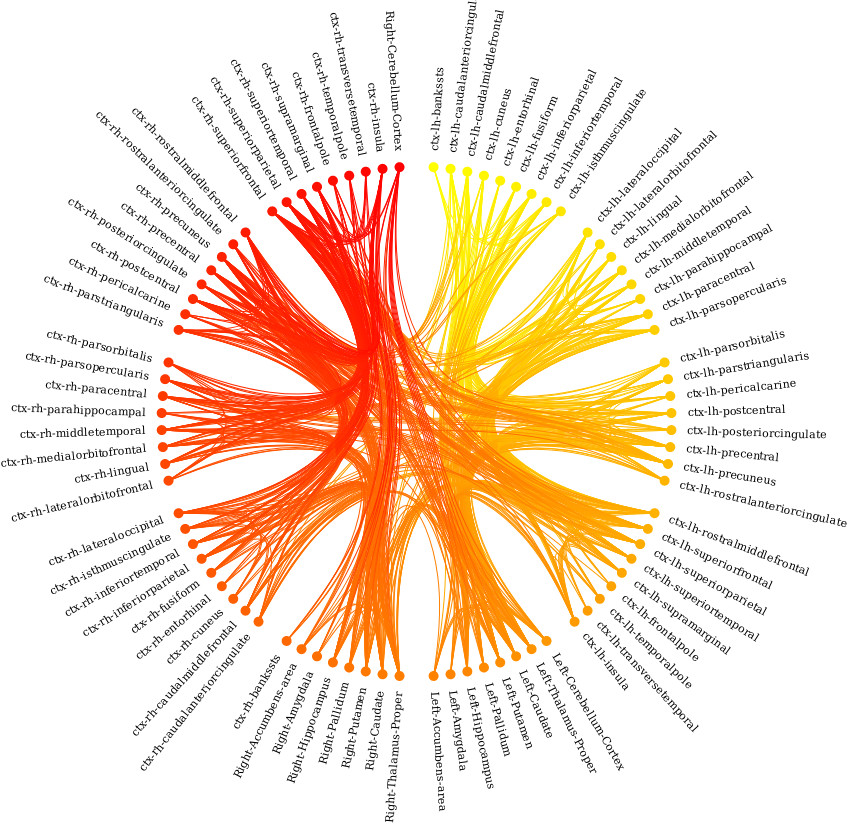
\includegraphics[width=\textwidth]{images/brain-data-viewer_2.png}
    %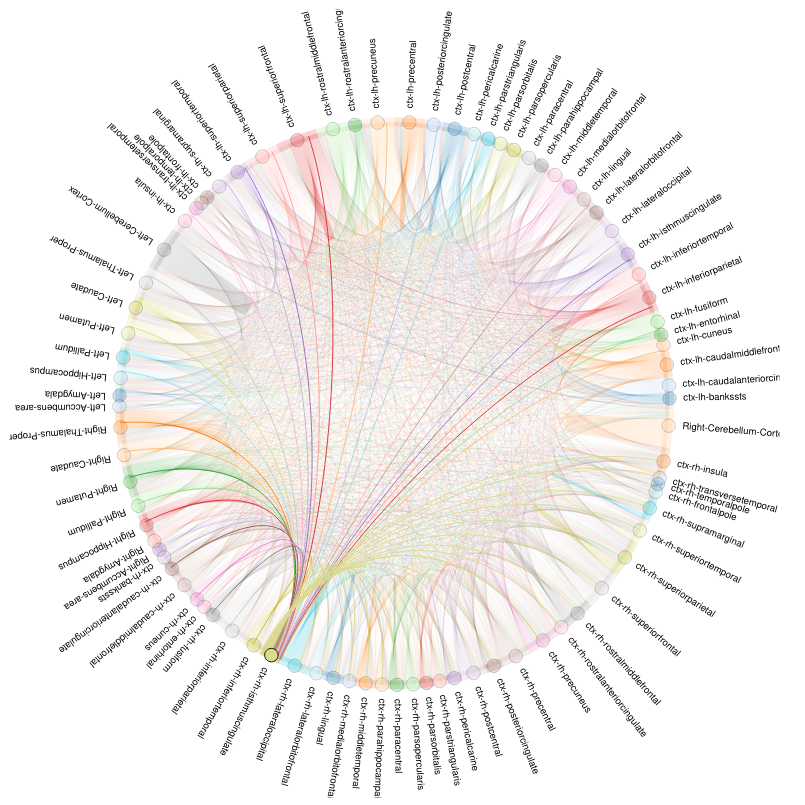
\includegraphics[width=\textwidth]{images/bokeh_plot_allsubjects.png}
    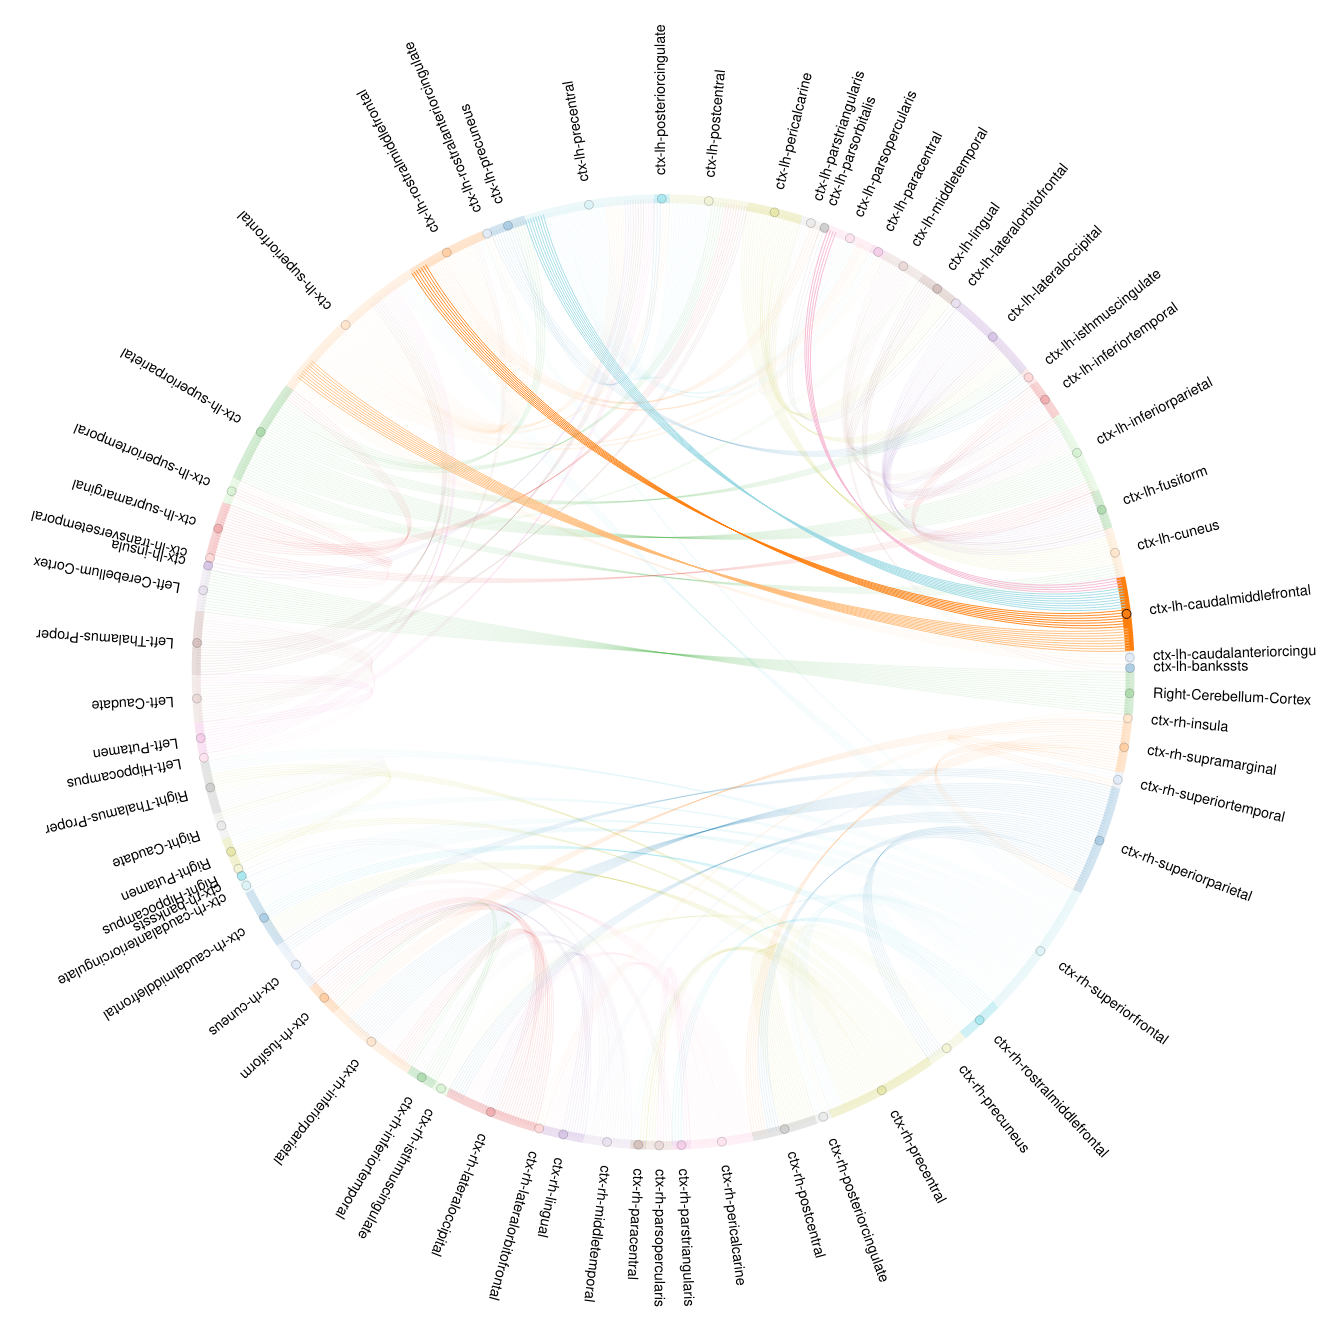
\includegraphics[width=\textwidth]{images/selected_view_all.png}
    \caption{A chord plot representing the group averaged connectome for all subjects. Nodes at the end of the circle correspond to grey matter \gls{ROI}s. The thickness of each edge corresponds to the number of arcs between two \gls{ROI}s. The number of arcs is proportional to the number of streamlines. In this interactive visualization the selected node (middle frontal gyrus in the left hemisphere) and its correspoding edges are highlighted while the other proprieties are made transparent. Edges connecting the selected node and target nodes are colored according to the target nodes. For example, the arcs are blue colored when there are connections to the precuneus in the left hemisphere.}
    \label{fig:connectome_num_streamlines}
\end{figure}

After the connectivity matrices for all subjects were generated using the methods in \autoref{sec:creating_connectome}, the group averaged connectome was created. The raw connectivity matrix was dense, containing $n = 84$ nodes and $n_e = 3486$ edges. The edge weights had high standard deviations for all the three connectivity metrics: mean FA, mean streamline length and number of streamlines. Visualizing the connectome as a simple connectivity matrix or a heatmap was hence not an effective strategy.

A chord plot was chosen because of the ease of representing grey matter nodes along the boundaries of the graph. The number of streamlines could also be encoded within a chord plot since the number of arcs drawn between any two nodes can be easily specified. The reason for the selection of the number of streamlines as a valid connectivity metric will be presented in \autoref{subsec:connmetric}. Furthermore, the detailed coloring scheme used for creating the chord plot gives added visual cues about the source and the target nodes. Once a node is selected the edges get colored according to the color of the target node.

In the chord plot represented in \autoref{fig:connectome_num_streamlines} $n=65$ nodes are shown. All nodes were colored to the color palette in \textit{holoviews}, with each node getting a different color. The graph is obtained by thresholding the group averaged number of streamlines between any two ROIs. The threshold was selected to be $N=900$. So only the connections which have more than $900$ streamlines would be selected. The plot represents the number of streamlines along the preserved connections scaled down by a factor of $10$ for ease of representation.

For interactive visualization, the cortical region caudal middle frontal in the left hemisphere is selected. Its has prominent connections to the cortical regions superior frontal, rostra middle frontal and precuneus in the left hemisphere. Weak connection to the cortical region parsopercularis is also well represented by this diagram. 

Overall, this comprehensive diagram is a systematic representation of whole brain connectivity. It can be used to analyze brain connections at the subject level or the group level.

\section{Feature Analysis}
\label{features}
Once the connectivity matrices were ready, it was important to investigate an effective connectivity metric and determine importance of within ROI connections. From the preprocessing pipeline presented in \autoref{subsec:connectomegeneration} there were three types of connectivity metrics obtained for each subject. These were number of streamlines, the mean streamline length and the mean FA. Each of these features encodes a different biological property of ROI-to-ROI connections and gave different classification results. There is no current consensus on which feature qualifies as an effective measure of connectivity between any two nodes \citep{yeh2020mapping}. The number of streamlines was selected to be the major focus of the classification tasks due its superiority in classification performance, which will be illustrated subsequently. Further, exclusion of self loops from the connectivity matrices will be experimentally justified. 

\subsection{Differences in connectivity metric}
\label{subsec:connmetric}
\begin{figure}
    \centering
    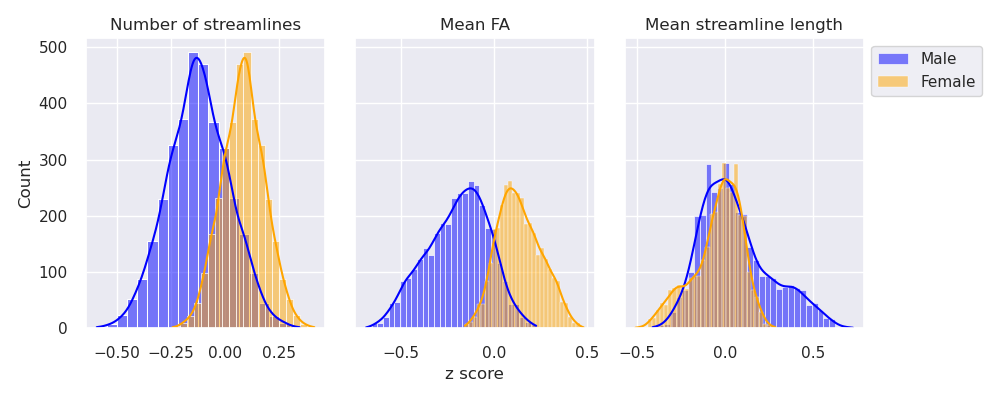
\includegraphics[width=\textwidth]{images/zscoredist.png}
    \caption{Three overlaid histograms representing the frequency of mean z-scores for different types of features. The orange histograms are for females and blue ones are for males.the y axis represents the number of between ROI connections.}
    \label{fig:hist_zscores}
\end{figure} 
As mentioned above, it was important to explore different types of connectivity metrics obtained from the connectivity matrices constructed using the methodology \autoref{fig:connectivity_matrix}. Considering the z-score distributions of \gls{ROI} connections separately for males and females was taken as a method for data evaluation. A histogram for the three different feature or connectivity types could help speculate how well they could separate between the two classes.

The histograms were formed using data (containing both data samples from males and females) in the training set. Each feature was then standardized by removing the mean and scaling it to unit variance. After scaling the feature value for each subject is represented by a z statistic. The mean of the z statistic (of one feature) is zero for all training subjects. However, the differences are prevalent when separate means are taken for the two genders. For each connection, there was one z-score for males and another for females depending on the connectivity metric. For each connectivity metric there are 3486 features which help form the distribution represented in \autoref{fig:hist_zscores}.

From the distributions, it is evident that the number of streamlines is a good metric for gender classification. It's histogram is shows a smooth Gaussian distribution for males and females, and has significantly higher peaks than those for the other two features. Even though the mean FA features have a smaller overlap visually, the variance of these histograms is high.

From the differences in z-score distribution, it can be inferred that women on an average have more number of streamlines as compared men, for the same connections. This observation is coherent with evidence in \cite{szalkai2015graph} showing that women have more densely connected brains than men. Further, women have higher white matter to grey matter ratio and hence the number of streamlines detected for women is higher \citep{taki2011correlations}.

The mean \gls{FA} plots illustrate that women have higher mean FA values than men. Conversely, an opposite trend is seen in the case of mean streamline length. Women have lower z-scores, which points that shorter streamline lengths. Currently, there are no conclusive results for benchmarking such a distribution as gender differences prevail depending on ROIs being considered \citep{kanaan2012gender}. For the mean FA, it is difficult to conclude that female brains have higher FA values since existing studies in whole brain connectivity do not provide conclusive results \citep{ingalhalikar2014sex}. The shorter streamline lengths in women seem plausible, on average women's brains are smaller than that of men \citep{ankney1992sex}.

The results for the number of streamlines and the mean streamline length are coherent with \textit{a priori} knowledge and evidence in literature. These features could have contained biases as the tractography was carried out in individual subject's space. Such biases were corrected for comparing the streamline count or length for different subjects using informed filtering from the SIFT algorithm (\cite{yeh2020mapping}).

The experiments stated above help establish the effectiveness of streamline count as a connectivity metric. It can discriminate well between gender and gives a biologically coherent measure of brain connectivity.

\subsection{Self loops}
\label{res:selfloops}

\begin{table}
\begin{tcolorbox}
\begin{tabular}{|p{0.135\textwidth}|l|l|l|l|}
\specialrule{0.2em}{0.01em}{0.01em}
\textbf{Label}& \textbf{ Metric}&\textbf{Feature}&\textbf{T statstic }&\textbf{P value}\\
\specialrule{0.2em}{0.1em}{0.1em}
Personality &Balanced&Mean FA&-0.196&0.846\\
Traits&accuracy&Mean streamline length&0.156&0.876\\
&&Number of streamlines &-1.248&0.217\\
&Area under &Mean FA&0.071&0.944\\
&ROC curve&Mean streamline length&1.332&0.188\\
&&Number of streamlines&-1.42&0.161\\
\specialrule{0.1em}{0.1em}{0.1em}
Gender&Balanced&Mean FA&0.396&0.695\\
&accuracy&Mean streamline length&2.068&0.048\\
&&Number of streamlines&0.98&0.335\\
&Area under &Mean FA&0.491&0.627\\
&ROC curve&Mean streamline length&3.875&0.001\\
&&Number of streamlines&2.199&0.036\\
\hline
\end{tabular}
\caption{Results for a paired samples t-test on the test set. The paired samples are the classification metrics of the data with and without the inclusion of self loops. The p values correspond to t-test of two arrays for the same classification metric constructed using methodology in \autoref{sec:exclusion}.}
\label{table:selfloops_combined}
\end{tcolorbox}
\end{table}

Evaluation of the importance of self loops was carried out on the basis of the experiment mentioned in \autoref{sec:exclusion}. The results in \autoref{table:selfloops_combined} were obtained by training the baseline experiments with and without the exclusion of self loops.  The report values correspond to classification performance on the test data. A positive t-statistic in this case indicates that the classification performance is greater with the inclusion of self loops. Meanwhile,  a negative t-statistic indicates the opposite trend. Statistical inference on this data indicates that the exclusion of self loops from the data analysis does not have a statistically significant effect on classification accuracy.  The statistics obtained from the analysis of both the target labels, i.e. the personality traits and gender labels do not lie in a significant confidence interval. The p-values in \autoref{table:selfloops_combined} are indicative of these results with most of them $p > 0.05$. 

Consider the statistics for the mean FA feature. All the p-values are $p>0.05$ and the t-statistic has opposite signs when it comes to considering two cases for personality classification. The first being balanced accuracy and the second as the area under the ROC curve. The t-statistic for the first case is $t=-0.196$ and for the second case is $t=0.071$. This opposite trend for two different  measures is indicative of the fact that there is no general trend of classification performance. 

With this investigation it became clear that the self loops can be eliminated from the data of all subjects. This ensured that the MEWS solver based technique as well as the baseline filters features from the same set of raw data.

\section{Baseline analysis}
\begin{figure}
    \centering
    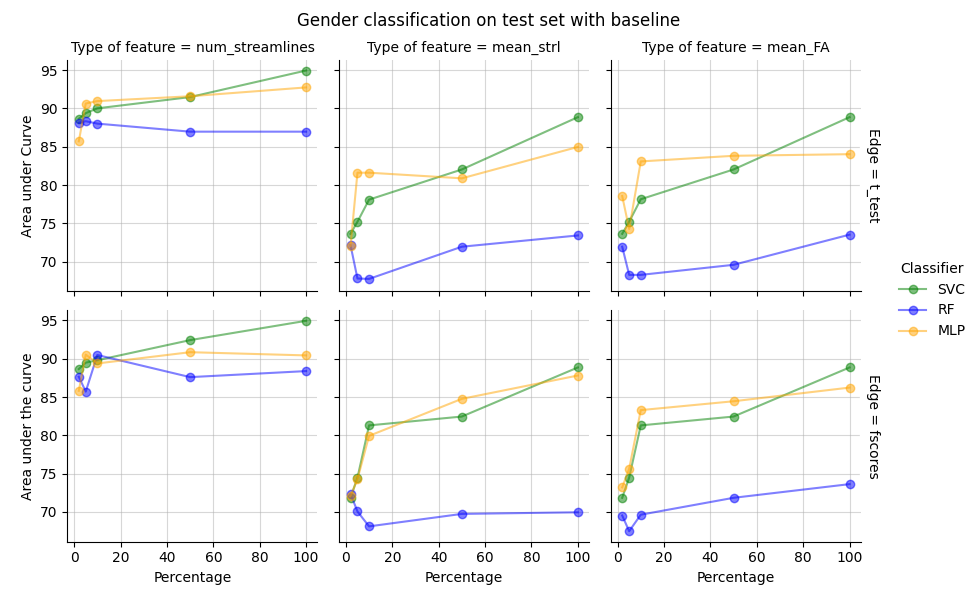
\includegraphics[width=\textwidth]{images/baseline_results_gender.png}
    \caption{Baseline analysis for gender classification. The area under the curve represented as a function of percentage of features. }
    \label{fig:baselinegender}
\end{figure}
\begin{figure}
    \centering
    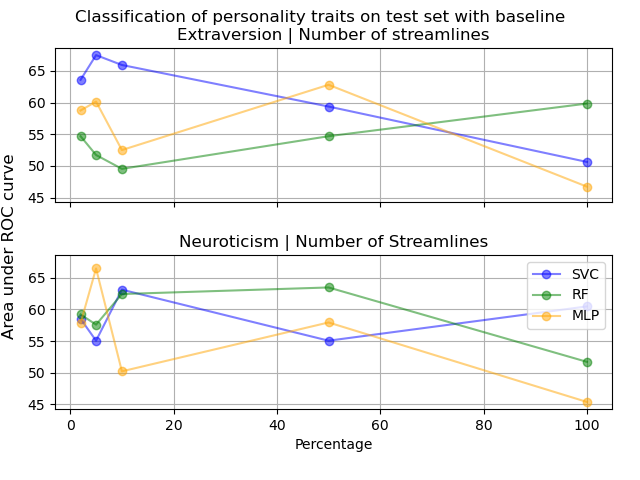
\includegraphics[width=0.8\textwidth]{images/persona_2.png}
    \caption{Baseline analysis on the basis of personality traits using pearson correlation coefficient as a filter method. For neuroticism, there is a trend of increase in performance with only a subset of original features using all three classifiers. The trend for the \gls{MLP} shows greater than 65\% area under ROC curve for top 5\% of features while 45\% without any feature selection. Classification performance on extraversion label increases with decrease in the number of features for classification with MLP and SVC. The strongest trend seen with the SVC, the area under ROC curve increases from 50\% (without feature selection) to around 67\% (using top 5\% of the original features). The overall trend for neuroticism and extraversion illustrates that it is useful to do some feature selection in order to predict these traits.}
    \label{fig:persona base}
\end{figure}
The baseline analysis mentioned in \autoref{subsec:Baseline_ana} with the parameter $k \in \{2,5,10,50,100\}$ was chosen to select the best performing connectivity metric. Here, $k$ denotes the percentage of features to be preserved. One important research question to be explored with this analysis was to determine whether doing any feature selection gives an added advantage to the classification accuracy.

From \autoref{fig:baselinegender}, it became evident that the number of streamlines served as a good metric for gender classification. There was only a loss of around 5\% performance for area under ROC curve while reducing the percentage of features from 100\% to 5\% for both types of edge representations, i.e. the t-test and f-scores and all three classifiers. In terms of number of features this meant that even choosing 175 out of 3486 features, most of the discriminative information could be preserved.

The baseline analysis of the different personality traits was more complex as compared to gender classification. All the possibilities of connectivity metrics and five different personality traits were considered in the pipeline. However, an overall trend could be observed only with neuroticism and extraversion. For these two personality traits, feature selection lead to much improved classifier performance with all three classifiers. A steep increase can be seen for extraversion where the area under ROC curve increases from about 50\% (random chance) to about 68\%.

For both the personality traits and the gender based classification, feature selection is profitable. In case of gender classification, an interpretability-performance trade-off was observed. This tradeoff is between the increase in interpretability with the decrease in the number of preserved features and decrease in classifier performance with the decline in the number of features. For personality classification the feature selection leads to a clear increase in interpretability and performance.

\section{Tracing back to original features}
A major motivation behind implementing the MEWS based technique for this thesis was interpretability of the feature selection. In this section the interpretability of the set of features selected by the baseline as well as the solver based implementation are compared. It is observed that the solver based method is superior to the traditional baseline method due to connectedness of the output features. 

The two subsequent subsections present visualizations for the features selected by both the feature selection techniques. Furthermore, the \autoref{subsec:solverfeat} provides an insight into how the solver implementation preserves edges. 
\subsection{Solver features}
\label{subsec:solverfeat}
For classification with the solver based technique detailed in \autoref{sec:MEWS}, the number of nodes preserved could be specified using a parameter $m$. Determining the order of growth in the number of edges as a function of $m$ was important to trace back the MEWS selected features to the original dataframe. \autoref{fig:fun_num_edges} shows a quadratic form with the number of edges $y$ as a function of the number of nodes $x$. This behavior is expected as the graph is supposed to be connected; i.e. there exists an edge between any two nodes in the graph. Using these results, the extent of interpretability from the solver results could be controlled. 
\begin{figure}
    \centering
    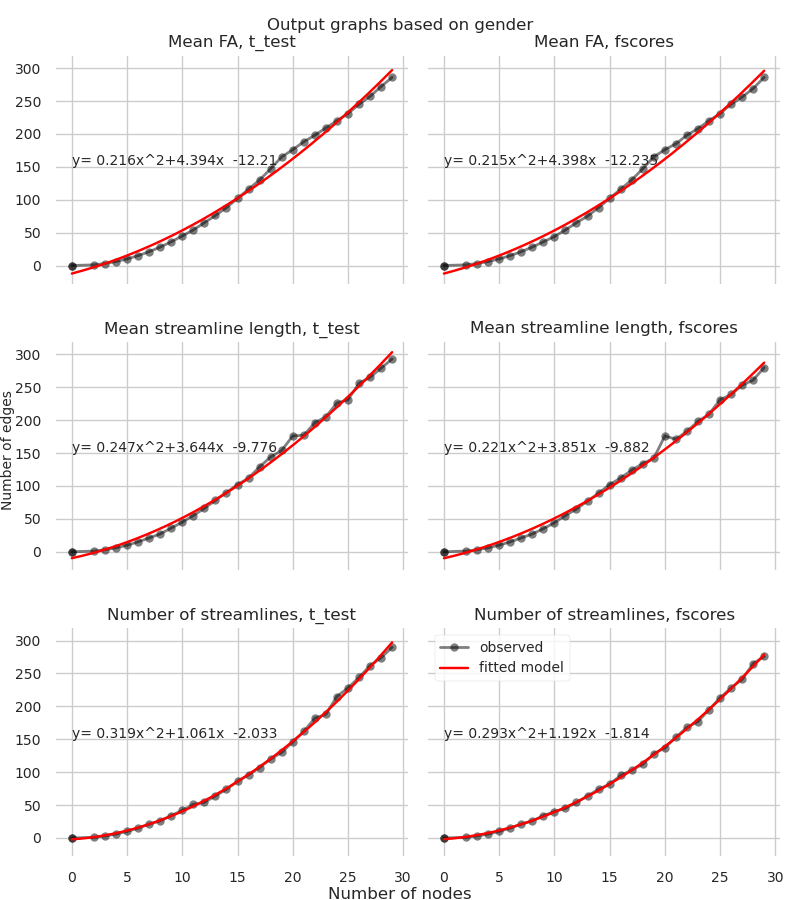
\includegraphics[width=0.7\textwidth]{images/Gender_nodes_preserved.png}
    \caption{Edges preserved as a function of the number of nodes supplied.}
    \label{fig:fun_num_edges}
\end{figure}

\subsection{Baseline Solver comparison}
\begin{figure}
    \centering
    %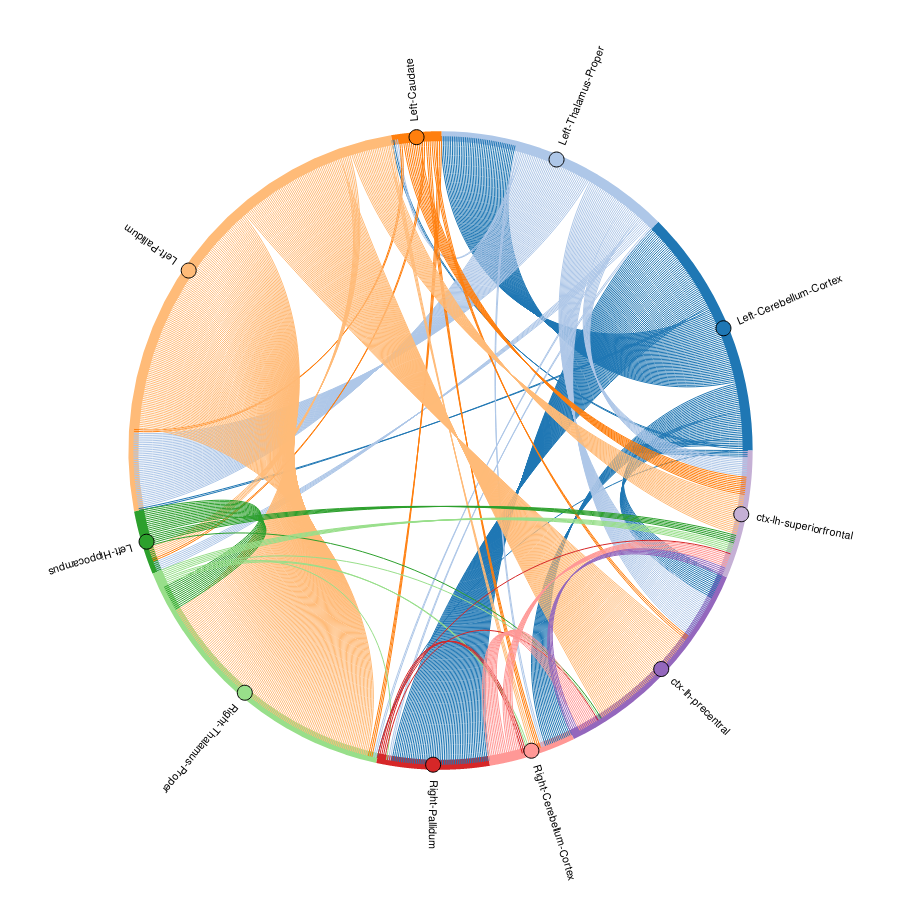
\includegraphics[width=0.9\textwidth]{images/gender10nodes_numstrls.png}
    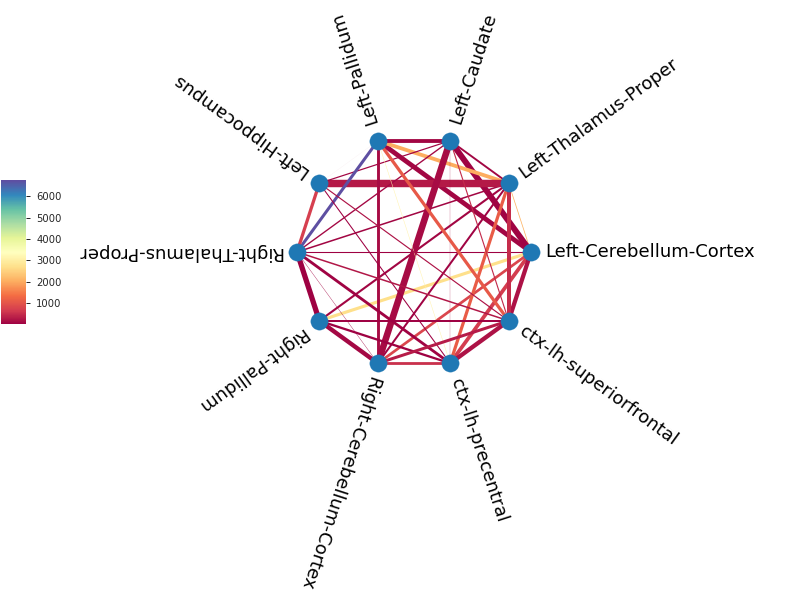
\includegraphics[width=0.7\textwidth]{images/solver_10nodes_strls.png}
    \caption{10 most important nodes determined using the solver based analysis for gender classification. The edge widths represent the f-scores of that edge and color represents the number of streamlines between the two regions.}
    \label{fig:gender_num_strls_10}
\end{figure}

\begin{figure}
    \centering
    %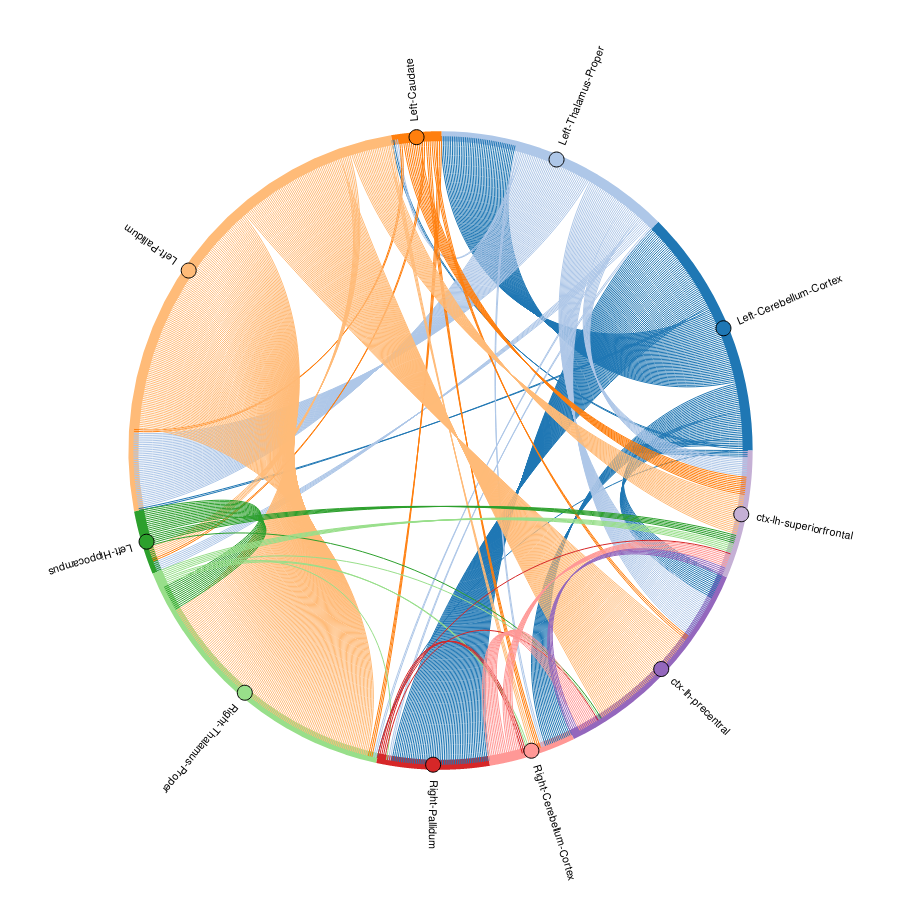
\includegraphics[width=0.9\textwidth]{images/gender10nodes_numstrls.png}
    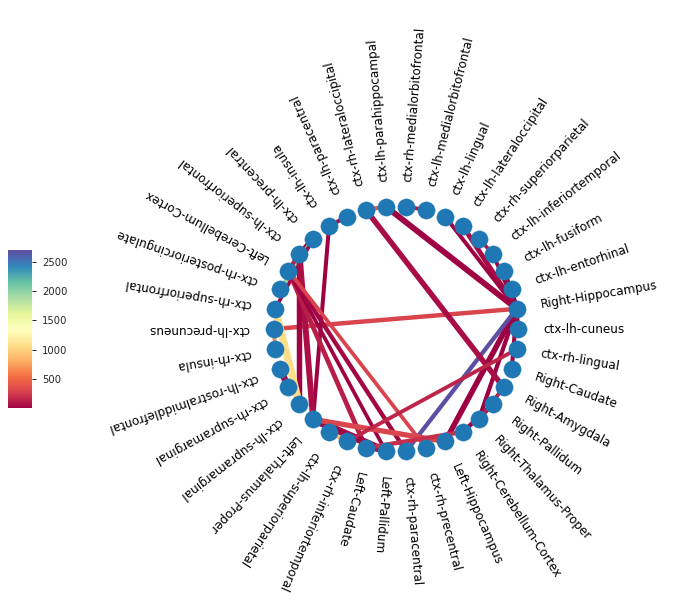
\includegraphics[width=0.9\textwidth]{images/baseline_42f_10nodes.png}
    \caption{41 most important features, and consequently 38 nodes preserved using baseline analysis for gender classification. The edge widths represent the f-scores of that edge and color represents the number of streamlines between the two regions.}
    \label{fig:baseline_num_strls_10}
\end{figure}

In order to compare the two feature selection techniques, a separate input graph had to be created for a two use cases according to \autoref{tab:classify_combo}. These two use cases were visualized to compare the interpretability of predictions from the solver and baseline analysis.

In the first use case, the type of feature is number of streamlines, the target label is gender, edge representation is f-score and feature selection is solver with 10 nodes preserved in the subgraph. In the second use case, all the parameters were the same as the first use case except for baseline as the feature selection technique and number of edges as 41 for comparison with 41 edges preserved in the first use case (using polynomial in \autoref{fig:fun_num_edges}). 

In both \autoref{fig:gender_num_strls_10} and \autoref{fig:baseline_num_strls_10},  the number of streamlines are group averaged for the training set and f-scores are also determined on the training data only. In \autoref{fig:gender_num_strls_10} the MEWS solver based implementation reduces the input graph and preserves 10 nodes along with 41 edges. It can be seen that the graph is well connected and structured .8 out of 10 most important nodes are subcortical regions. One inference that can be drawn from this visualization is that gender differences might be more prevalent in subcortical regions than cortical ones since the edge widths as well as number of streamlines for subcortical regions are higher. \autoref{fig:baseline_num_strls_10} illustrates that for the same number of edges (41) there are 38 nodes preserved. The graph is not connected and there are isolated edges. 

\autoref{fig:gender_num_strls_10} and \autoref{fig:baseline_num_strls_10} illustrate the superiority of the MEWS solver generated subgraphs over baseline features in terms of interpretability. In a research setting, the MEWS solver method would hence be more beneficial since it provides more interpretable results. With this technique it becomes easier to determine the subnetworks related to a particular target variable. 


\section{Model performance}

\begin{figure}
    \centering
    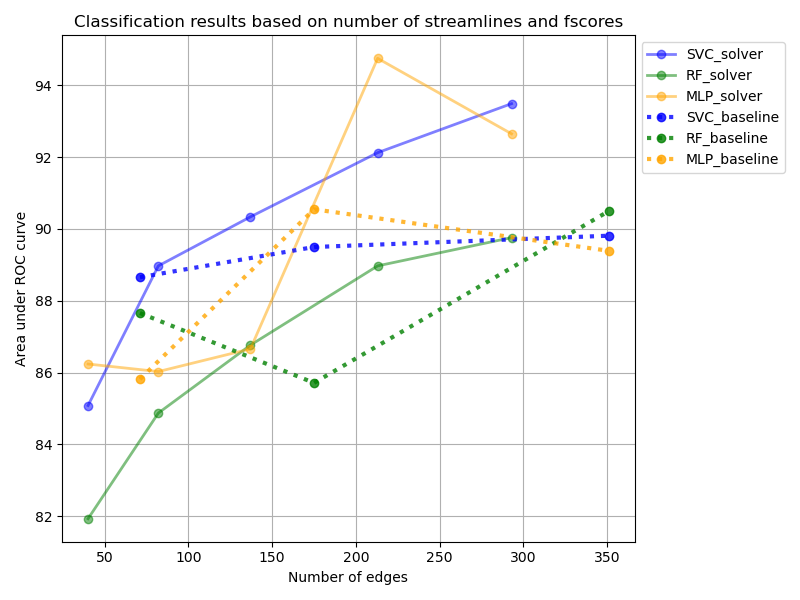
\includegraphics[width=0.8\textwidth]{images/select_clf_auc_gender.png}
    \caption{Comparison of area under the ROC curve for gender classification on the independent test set. The performance of three classifiers \gls{SVC}, \gls{RF2} and \gls{MLP} on the basis of features filtered according to the solver and baseline experiments respectively.}
    \label{fig:clf_solver results}
\end{figure}

\begin{figure}
    \centering
    %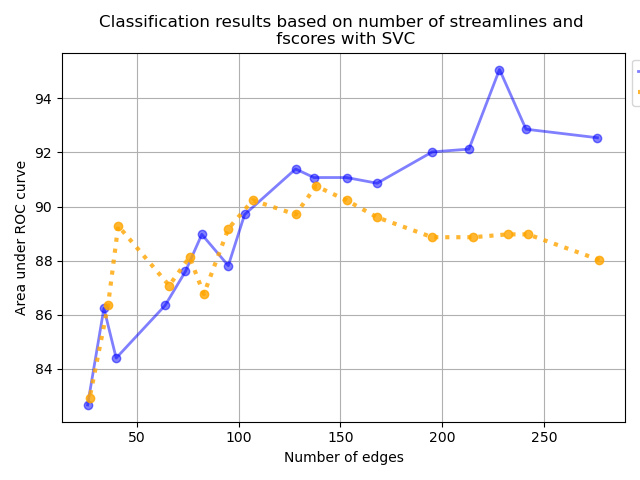
\includegraphics[width=0.8\textwidth]{images/select_clf_auc_gender_2_svc.png}
    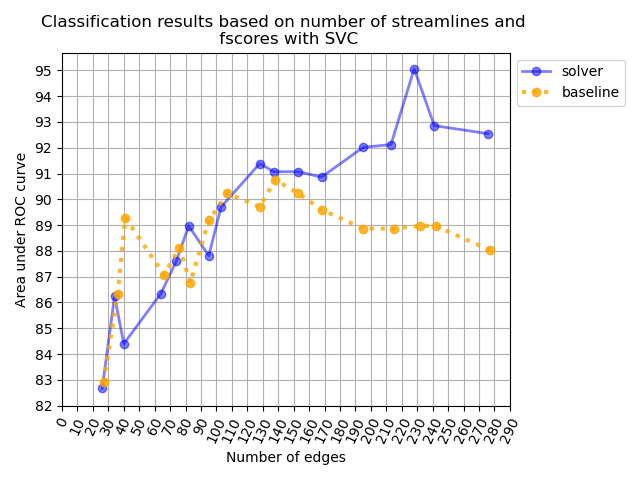
\includegraphics[width=0.8\textwidth]{images/select_clf_auf_gender_2_scaled.png}
    \caption{Gender classification using solver and baseline for the exact same number of features selected in each case.}
    \label{fig:svcgender}
\end{figure}
Classification performance on the target label varied depending on the parameters of the data given to the classifier according to \autoref{tab:classify_combo}.

For the classification of gender, the comparison of classification performance was easily interpretable. At first, the baseline experiments for $k \in \{2,5,10\}$ were compared with solver nodes $m \in \{5,10,15,25,30\}$ due to computational complexity of the exhaustive search. \autoref{fig:clf_solver results} was used to determine the which classifier performs the best and gives results free from overfitting. 

The SVM based classification produced the most stable results out of the three classifiers used. 
One the classifier was decided upon, classification performance for a higher number of data points were then sampled. This time the number of edges preserved by the solver was used to decide the parameter top $k$ percentile of features to be preserved in the baseline analysis. 

The subsequent results in \autoref{fig:svcgender} clearly indicate a cutoff number of edges, i.e. precisely 137 (obtained from the function in \autoref{fig:fun_num_edges}). The MEWS solver definitely does better than the baseline analysis in terms of classification performance. Even for the number of edges below 137, the results remain comparable. 

It can be inferred that using the \gls{MEWS} solver, after 137 edges or 20 nodes (using \autoref{fig:fun_num_edges}). In summary, for gender classification preserving less than 20 nodes leads a reduction in classifier performance but an increase in ease of visualization and interpretability. With $m> 20$ nodes, there is a decrease in interpretability but an increase in classifier performance.

\begin{figure}
    \centering
    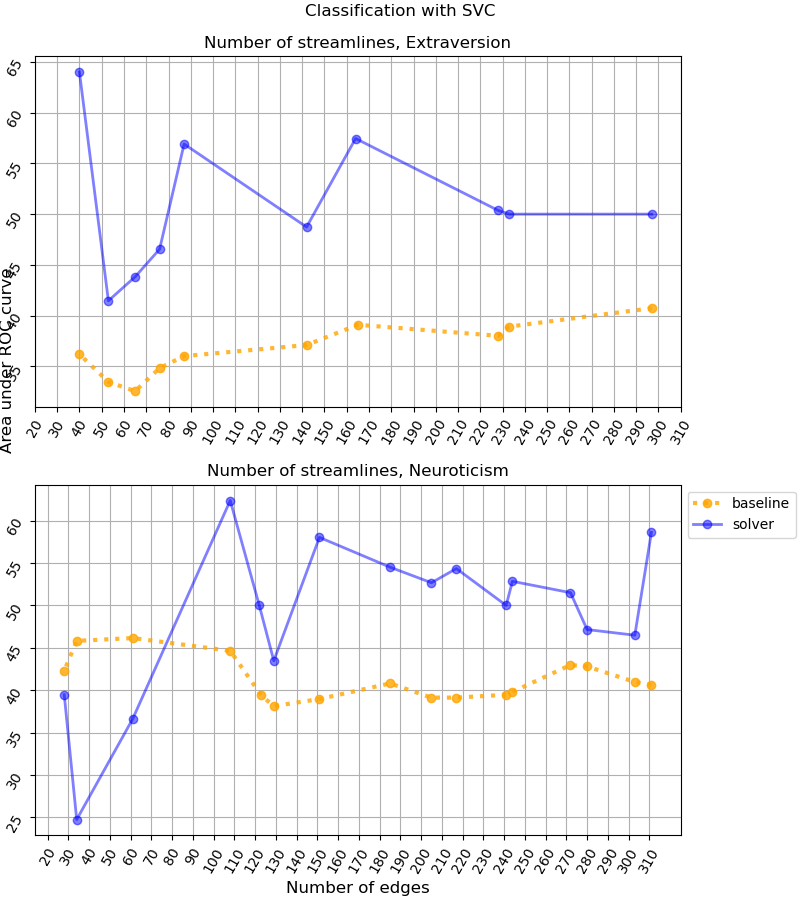
\includegraphics[width=\textwidth]{images/persona_comp.png}
    \caption{Comparison of solver and baseline for classification of personality traits.}
    \label{fig:persona_com}
\end{figure}

\subsection{Best parameters}

\iffalse
For our configuration using Multilayer perceptron for the solver based reduction, classification of gender using the feature selection technique of f-scores and refit metric balanced accuracy. Baseline based on 5\% of features. The parameters for the best estimator of the cross validation turn out to be the same, this justifies that the solver based method works better than the baseline method when it comes to classification accuracy and also leads to an increase in the interpretability.
% Best estimator {'solver': 'adam', 'learning_rate': 'adaptive', 'hidden_layer_sizes': (50, 100, 100, 50), 'alpha': 0.05, 'activation': 'relu'}
% ('MLP', 'Gender', 'random', 'f-scoress', 'baseline', 'num_streamlines', 5, 'balanced_accuracy', False)
%Bet estimator {'solver': 'adam', 'learning_rate': 'adaptive', 'hidden_layer_sizes': (50, 100, 100, 50), 'alpha': 0.05, 'activation': 'tanh'}
\begin{table}[b]
    \centering
    \begin{tabular}{|c|c|c|}
        \specialrule{0.1em}{0.05em}{0.05em}
        Hyperparameter & Solver & baseline \\
        \hline
        solver & adam & adam\\
        \hline
        hidden layer size &  50,100,100, 50 & 50,100,100,50\\
        \hline
        activation function & relu & tanh\\
        \hline
        alpha & 0.05 & 0.05\\
        \hline
        learning rate & adaptive & adaptive\\
        \hline
    \end{tabular}
    \caption{Cross validation parameters for MLP trained for gender classification. The parameters which give the best area under the curve for the use case mentioned in the section above have been presented}
    \label{tab:MLP best params}
\end{table}
\fi
\begin{table}[h]
\begin{tcolorbox}
    \centering
    \begin{tabular}{!{\vrule width 2pt}c|c|c!{\vrule width 2pt}}
        \specialrule{0.2em}{0.01em}{0.01em}
        Hyperparameter & Solver & baseline \\
        \hline
        C & 5.9 & 0.522\\
        \hline
        Gamma &  4e-4 &  8e-4\\
        \hline
        kernel &  rbf & rbf\\
        \hline
        class weight & balanced & None\\
        \specialrule{0.2em}{0.01em}{0.01em}
    \end{tabular}
    \caption{Cross validation parameters for SVC trained for gender classification. The parameters which give the best area under the curve for the use case mentioned in the section above have been presented}
    \label{tab:CSV best parameters}
\end{tcolorbox}
\end{table}

The SVC gave most stable results as compared to other classifiers. In \autoref{tab:CSV best parameters} the parameters of the best estimators for the MEWS solver based method and baseline used for gender classification will be presented.

The best performing estimators are determined using \autoref{fig:svcgender}.For gender classification using the solver, the maximum area under ROC curve of 95\% for the independent test set could be achieved. This performance is obtained for 237 edges corresponding to 26 nodes. Using the baseline technique, the best estimator could achieve 91\% area under curve  for around 138 edges.
%Best estimator {'C': 5.918565074193836, 'class_weight': 'balanced', 'gamma': 0.0004643818614121193, 'kernel': 'rbf'}
%Best estimator basline {'C': 0.5229762127721259, 'class_weight': None, 'gamma': 0.008523831363402392, 'kernel': 'rbf'}



\end{document}
